\documentclass[11pt]{article}

% lpackage 
\usepackage{amsmath,amssymb,amsthm}
\usepackage{graphicx}
\usepackage{caption}
\usepackage{subcaption}

% margin
\addtolength{\evensidemargin}{-.5in}
\addtolength{\oddsidemargin}{-.5in}
\addtolength{\textwidth}{0.8in}
\addtolength{\textheight}{0.8in}
\addtolength{\topmargin}{-.4in}

% custom definitions
\newtheoremstyle{quest}{\topsep}{\topsep}{}{}{\bfseries}{}{ }{\thmname{#1}\thmnote{ #3}.}
\theoremstyle{quest}
\newtheorem*{definition}{Definition}
\newtheorem*{theorem}{Theorem}
\newtheorem*{question}{Question}
\newtheorem*{exercise}{Exercise}
\newtheorem*{challengeproblem}{Challenge Problem}
\newcommand{\name}{

%% put your name here, so we know who to give credit to %%
[Your Name Here]
}
\newcommand{\hw}{
%% and which homework assignment is it? put the correct number below        
1
}

\title{\vspace{-50pt}
\Huge \name
\\\vspace{20pt}
\huge POLSCI 514\hfill Problem Set \hw}
\author{}
\date{}
\pagestyle{myheadings}
\markright{\name\hfill Problem Set \hw\qquad\hfill}

%% If you want to define a new command, you can do it like this:
%% The followins is the useful commands for math and probability. 
\newcommand{\R}{\mathbb{R}}
\newcommand{\E}{\mathbb{E}}
\newcommand{\V}{\mathbb{V}}



\begin{document}
\maketitle



\section{Writing in math mode}
The most important thing is how to write down mathematical expressions in \LaTeX.
There are several ways to write equations. 

\subsection{Inline equation}
The first way is to enclose equations in dollar signs: $x+y=a^2+b^2$.
This is useful when you want to embed a simple equation in your text.

\subsection{One equation in a new line}
If you want to use new line for equations, there are two ways:

\[x+y=a^2+b^2\]

or

$$
x+y=a^2+b^2
$$

\subsection{Many equations in new lines}
If you have a chain of deductions, you can line them up like this.
The \& tells it where to line up---usually you will want it right before the equals sign.
You should have an 'and' symbol, \&, in each line.
The double-backslash, $\backslash\backslash$, means indentation. 
\begin{equation}
\begin{split}
  2x &= 2y-10 \\
  x &=y -5   \\
\end{split}
\end{equation}


If you don't want to enumerate the equations, add an asterisk:
\begin{equation}
\begin{split}
  2x &= 2y-10 \\
  x &=y -5  
\end{split}
\end{equation}

You might want to include words if they are short:
\begin{equation}
\begin{split}
  2x &= 2y-10 \quad \text{bla bla bla}\\
  x &=y -5  
\end{split}
\end{equation}


\subsection{Symbols}

There are some symbols that often come up in the homework. \\
\begin{itemize}
    \item $\mathbb{E}$: Expectation  
    \item $\mathbb{V}$: Variance
    \item $\mathbb{P}$: Probability measure
    \item $\mathbb{R}$: Set of real numbers
\end{itemize}
This is new area.

In this template, you can simply type $\E$, $\V$ and $\R$ (but not P becasue a backslash and P is already defined as $\P$.) 
See the header for the alphabets with this functionality. 

You can write Greek letters in the way they are read. $\alpha$, $\beta$, $\gamma$, 
$\lambda$, $\omega$. Capitalize the first letter to get the capital letters. $\Omega$

Other useful symbols are like this. 
\begin{itemize}
    \item $\cup$: union
    \item $\cap$: intersection
    \item $a \in A$ : $a$ is an element of $A$
    \item $A = \{1, 2, 3\}$: specify a set by its elements. 
    % For { }, you have to escape by a backslash. i.e. \{ \}
    \item $\mathcal{F}$: set of events
    \item $\sum_{i=1}^n$: summation 
    \item $\prod_{i=1}^n$: product 
    \item $\int_{x=0}^1$: integral 
    \item $\sim$: distributed as 
    % if you have more than one letter in sub/superscript, use {}.
\end{itemize}


\subsection{Matrix}

Plain matrix
\begin{equation}
\begin{matrix}
1 & 2 & 3\\
a & b & c
\end{matrix}
\end{equation}

Parenthesis
\begin{equation}
\begin{pmatrix}
1 & 2 & 3\\
a & b & c
\end{pmatrix}
\end{equation}

Square brackets
\begin{equation}
\begin{bmatrix}
1 & 2 & 3\\
a & b & c
\end{bmatrix}
\end{equation}



\subsection{Others}
\begin{itemize}
    \item superscripts: $X^2$ 
    \item subscripts: $X_2$ 
    \item both superscripts and subscripts: $X_2^2$ 
    \item both superscripts and subscripts: $X_2^2$ 
    \item fractions: $\frac{1}{x}$ 
    \item binomial: $\binom{1}{x}$ 
    \item Parentheses size: normal $()$, big $\big(\big)$, Big $\Big(\Big)$, Bigg $\Bigg(\Bigg)$
    \item Parentheses size (Alternative): left and right e.g. $\left[  \frac{ N } { \left( \frac{L}{p} \right)  - (m+n) }  \right]$ 
    \item three dots: $\ldots$ $\cdots$ e.g. $X = 1, \ldots, N$ 
    \item transpose: $X^{\intercal}$ vs $X^{T}$ 
    \item white space: $x\ y$, $x\quad y$, $x\qquad y$
    \item cases: 
      \begin{equation}
          Y = 
          \begin{cases}
            1 &\text{if}\quad Y^* > 0 \\
            0 & \text{otherwise} 
          \end{cases}
      \end{equation}
    \item infinity: $\infty$ 
    \item text on top of equation/symbols $X \stackrel{i.i.d}{\sim} Normal(0, 1)$
\end{itemize}

\subsection{Multiple line equations}
Some examples
\begin{equation}
\begin{split}
    f(x \vert p) &= \prod_{i=1}^n p^{x_i} (1-p)^{1-x_i} \\
    &= \exp\Big(\sum_{i=1}^n x_i \log p + (n-\sum_{i=1}^n x_i) \log(1-p)\Big) \\
    &= \exp\Big(\sum_{i=1}^n x_i (\log p + \log(1-p)) + n \log(1-p) \Big)
\end{split}
\end{equation}

\begin{equation}
\begin{split}
    &p(\pi, \eta \vert D, C^l) \\
    &\propto p(\pi) p(\eta) p(D^{lp}, C^{lp} \vert \pi, \eta) p(D^{ln}, C^{ln} \vert \pi, \eta) \Big[p(D^u \vert \pi, \eta)\Big]^{\lambda} \\
    &= p(\pi) p(\eta) 
    \times \prod_{i=1}^{N^{lp}} p(D_i^{lp} \vert Z_{ik^*}, \eta) p(Z_{ik^*} \vert \pi) \\
    &\quad \times \prod_{i=1}^{N^{ln}} \sum_{k \neq k^*} \Big\{ p(D_i^{ln} \vert Z_{ik}, \eta) p(Z_{ik} \vert \pi) \Big\} 
    \times \Bigg[\prod_{i=1}^{N^{u}} \sum_{k=1}^K \Big\{ p(D_i^{u} \vert Z_{ik}, \eta) p(Z_{ik} \vert \pi) \Big\} \Bigg]^{\lambda} \\
    &\propto \underbrace{\prod_{k=1}^K \pi_k^{\alpha_k - 1} \prod_{v=1}^V \prod_{k=1}^K \eta_{vk}^{\beta_k - 1}}_\text{prior}
    \times 
    \underbrace{\prod_{i=1}^{N^{lp}} \Big[ \prod_{v=1}^V \eta_{vk^*}^{D_{iv}}\times \pi_{k^*} \Big]}_\text{positive labeled doc. likelihood} \\
    &\quad \times \underbrace{\prod_{i=1}^{N^{ln}} \sum_{k \neq k^*} \Big\{ \prod_{v=1}^V \eta_{vk}^{D_{iv}}\times \pi_k \Big\}}_\text{negative labeled doc. likelihood} 
    \times \underbrace{\Bigg[\prod_{i=1}^{N^{u}} \sum_{k=1}^K \Big\{ \prod_{v=1}^V \eta_{vk}^{D_{iv}}\times \pi_k  \Big\}\Bigg]^{\lambda}
}_\text{unlabeled doc. likelihood}
\end{split}
\end{equation}

\newpage
\section{Inserting figures}


\begin{figure}[h!]  % Figure float begins. []: controls where the figure is placed
\centering % place the figure at the center in the float
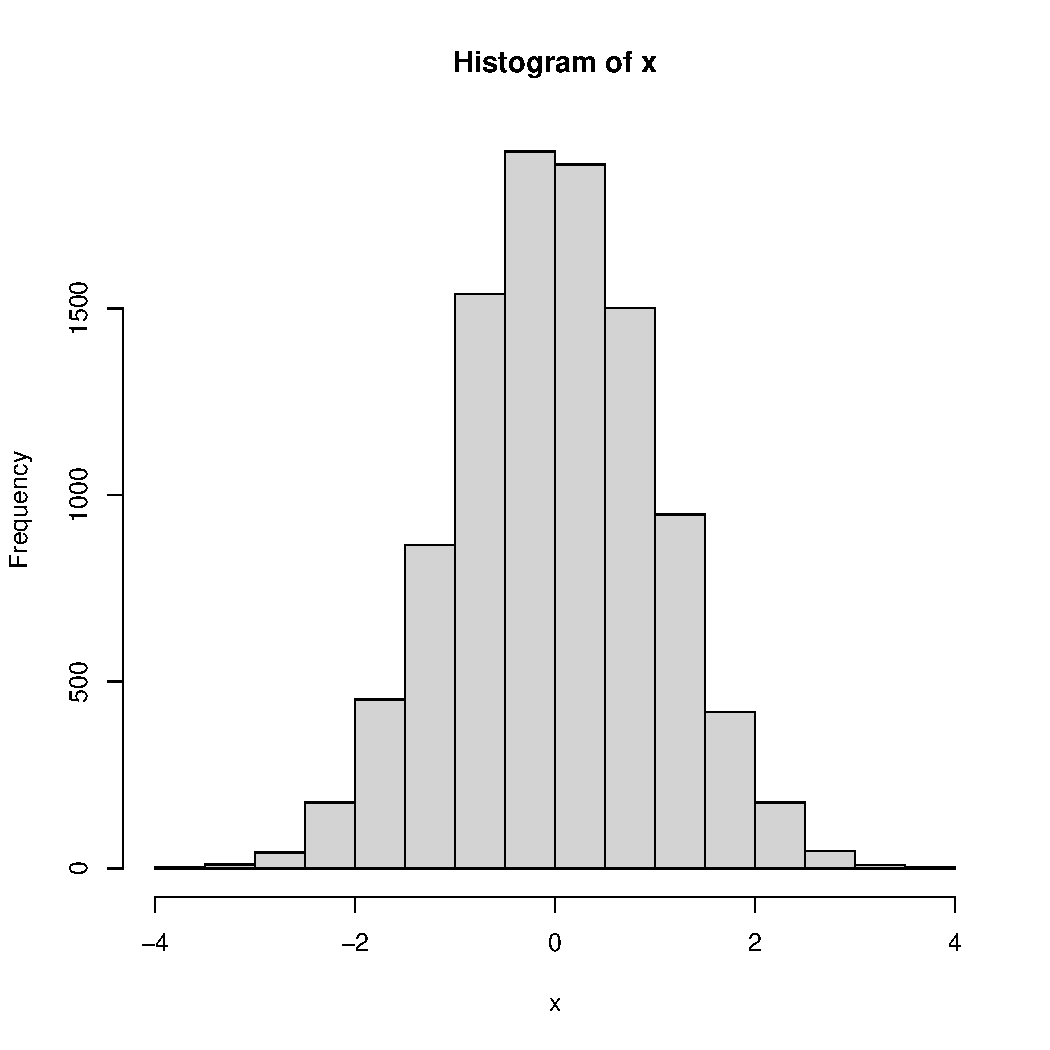
\includegraphics[scale=0.3]{figs/normal.pdf} % []: controls the size of the figure; {}: specifies the path to the figures
\caption{ % always add caption to the figure 
  Some caption here
}
\label{fig:normal} % label to be used when we reference the figure
\end{figure}

\subsection{Where to place figures}
The following parameters will control where the figure is placed.
\begin{itemize}
  \item h: here 
  \item t: top 
  \item b: bottom 
  \item p: place it in a page that only contains float (i.e. figures or tables)
  \item !: "please really respect my choices here" 
\end{itemize}

\subsection{The size of figures}
\begin{itemize}
  \item scale=1.5 : 1.5 times the real size 
  \item width=4cm, height=3cm: manually specify the width and the height 
  \item width=\textbackslash textwidth: the same width with the text width 
\end{itemize}

\subsection{Reference}
\begin{itemize}
  \item \textbackslash label\{fig:normal\}: define the name of the figure to be referenced 
  \item \textbackslash ref\{fig:normal\}: refernece the figure. e.g. Fig \ref{fig:normal} shows a histogram of ...
\end{itemize}



\begin{figure}[t]  
\centering 
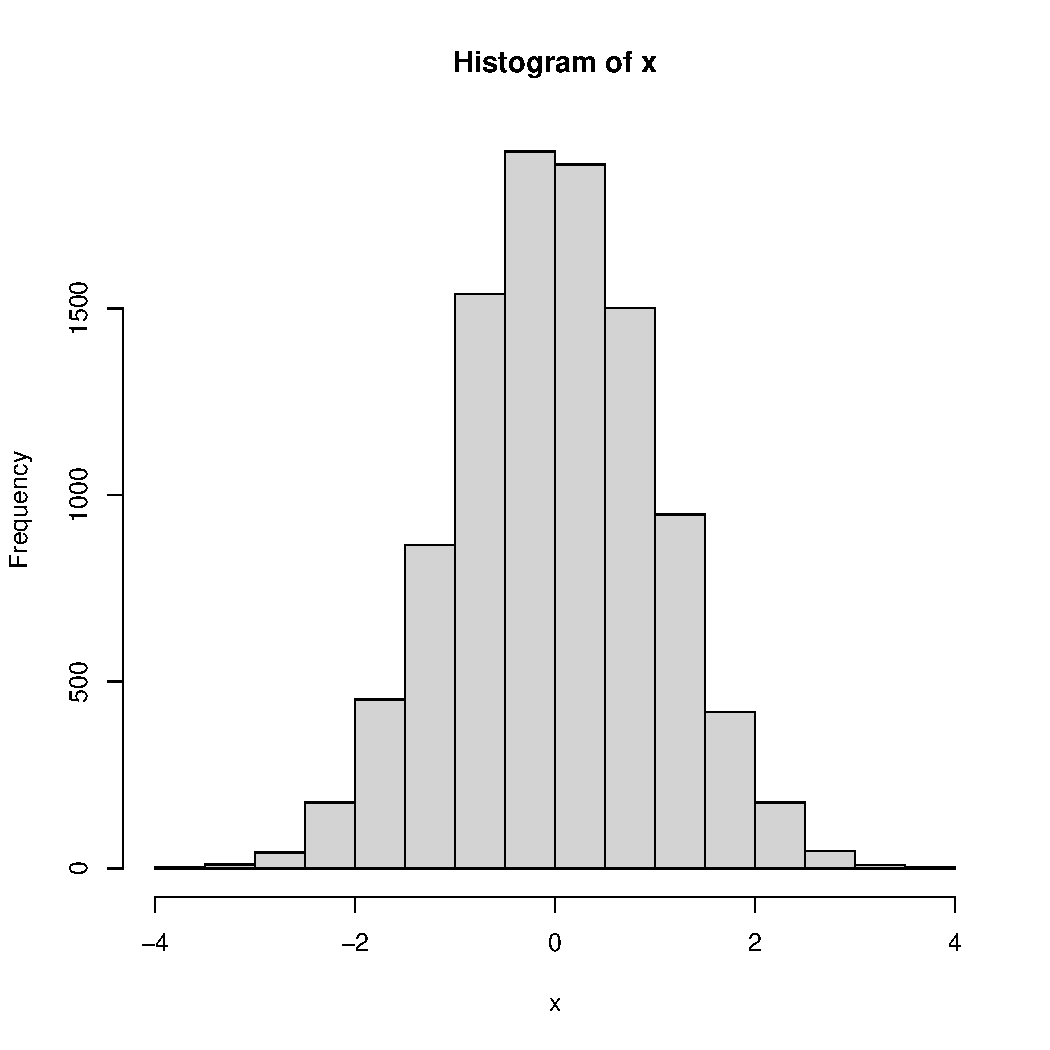
\includegraphics[width=\textwidth]{figs/normal.pdf} 
\caption{ 
  Top with text width 
}
\end{figure}

\begin{figure}[b]  
\centering 
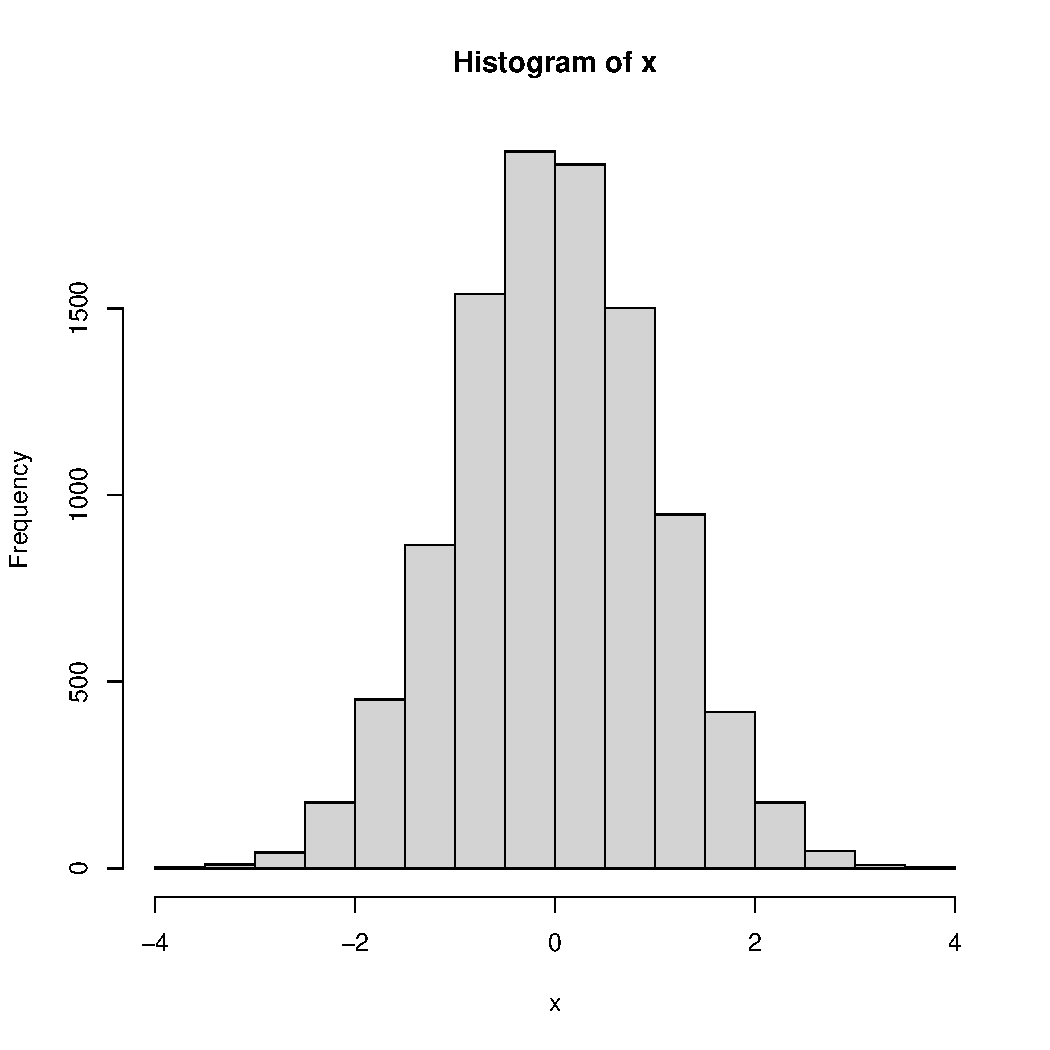
\includegraphics[width=3cm, height=4cm]{figs/normal.pdf} 
\caption{ 
  bottom with manual width and height
}
\end{figure}

\begin{figure}[p!]  
\centering 
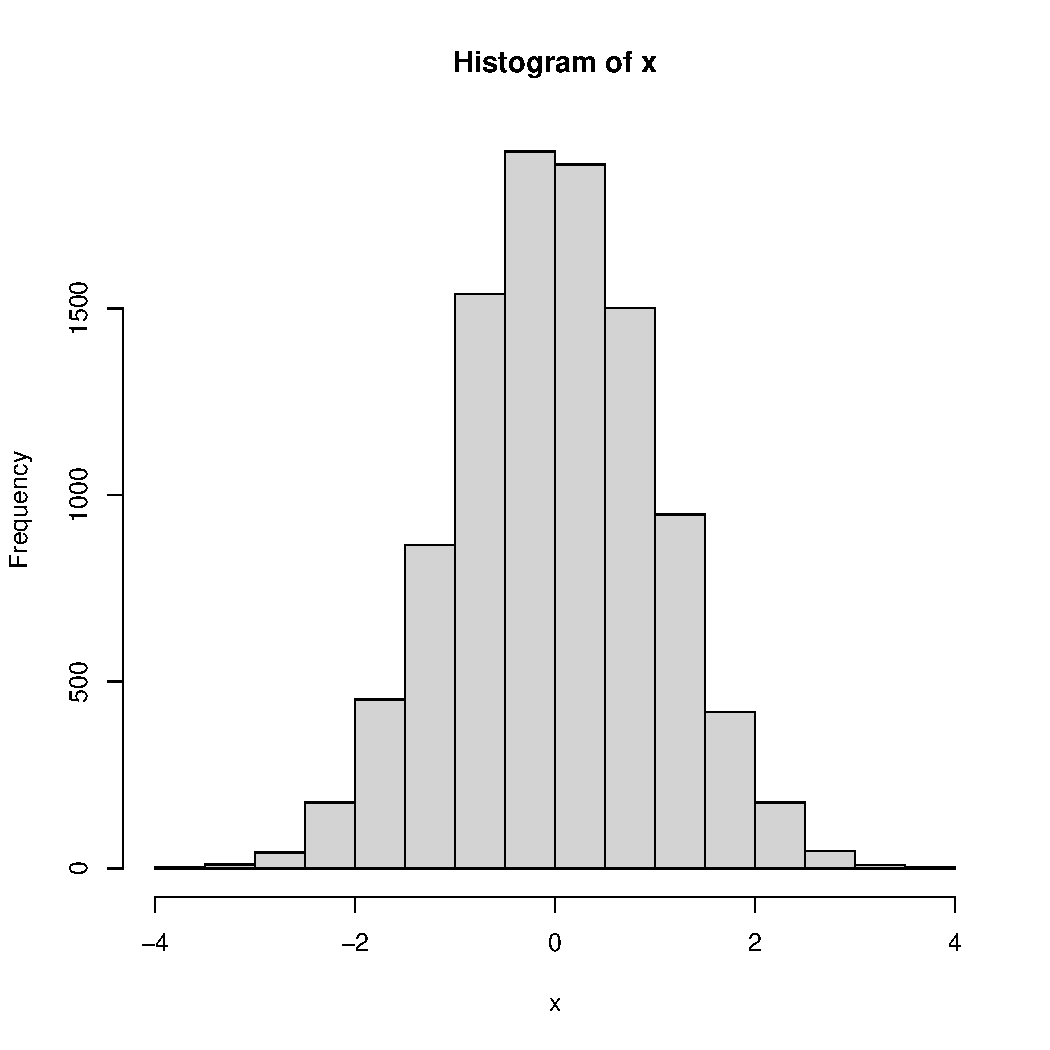
\includegraphics[scale=0.7]{figs/normal.pdf} 
\caption{ 
  page 
}
\end{figure}

\subsection{Multiple subfigures}
This requires two packages ``caption'' and ``subcaption''  
\begin{figure}
     \centering
     \begin{subfigure}[b]{0.3\textwidth}
         \centering
         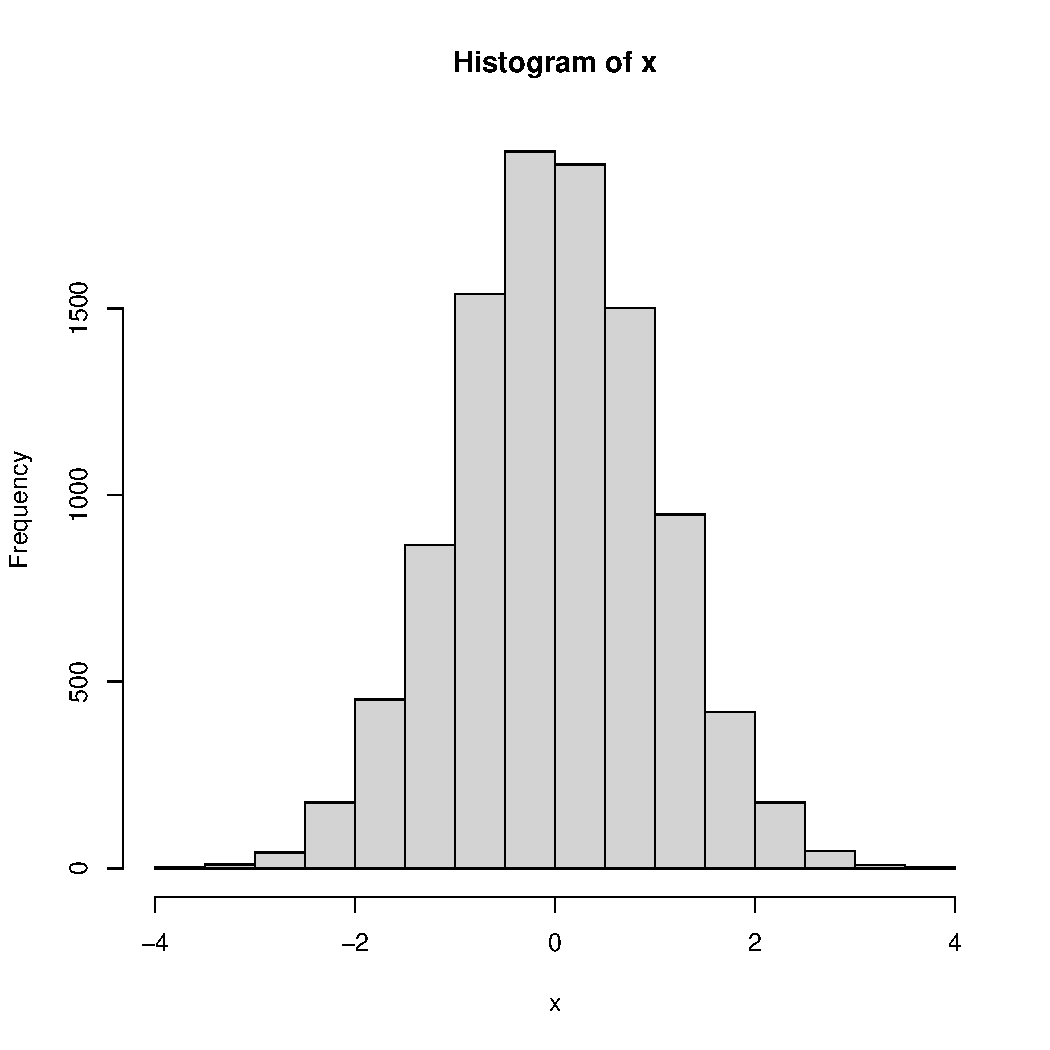
\includegraphics[width=\textwidth]{figs/normal.pdf}
         \caption{Normal}
     \end{subfigure}
     \hfill
     \begin{subfigure}[b]{0.3\textwidth}
         \centering
         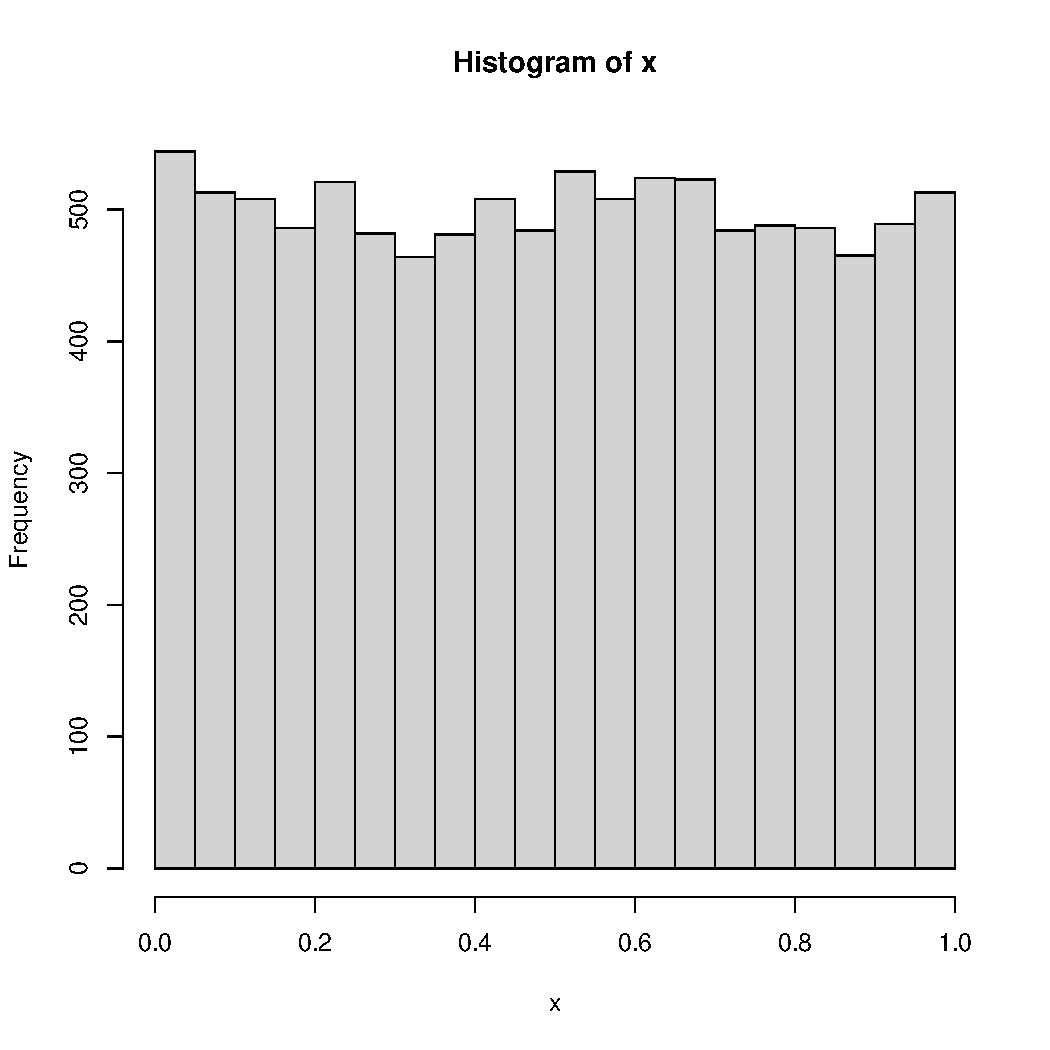
\includegraphics[width=\textwidth]{figs/unif.pdf}
         \caption{Uniform}
     \end{subfigure}
     \hfill
     \begin{subfigure}[b]{0.3\textwidth}
         \centering
         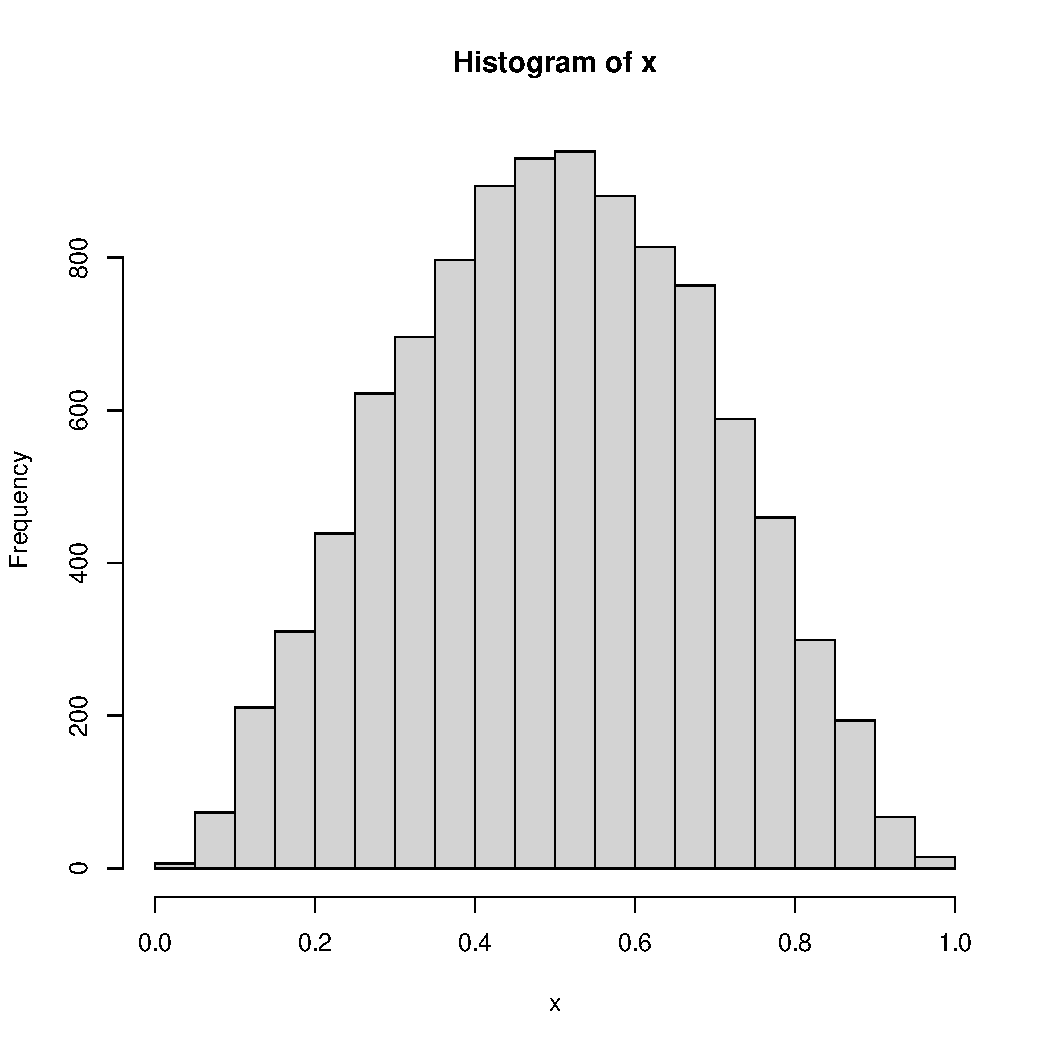
\includegraphics[width=\textwidth]{figs/beta.pdf}
         \caption{Beta}
     \end{subfigure}
        \caption{Three distributions}
\end{figure}


\clearpage % make sure that all the figures are placed within the section (c.f. \newpage doesn't assure this)
\section{Inserting tables}

Inserting tables are very similar to inserting figures.
An example of displaying summary statistics from a survey.


\begin{table}[h!] % start a float for a table
\centering
\begin{tabular}{ll|rr}
% NOTE: {l: left, r: right, c: center} will specify the location of text within a cell.
\hline
\hline
\textbf{Variable} & \textbf{Levels} & $\mathbf{n}$ & $\mathbf{\%}$ \\ 
\hline
Gender & Male & 1531 & 52.8 \\ 
   & Female & 1411 & 47.8 \\ 
   & Other & 1 & 0.0 \\ 
   & NA & 11 & 0.4\\
\hline
\hline
Age & 19-30 & 474 & 16.0 \\ 
   & 30-40 & 597 & 20.2 \\ 
   & 40-50 & 704 & 23.8 \\ 
   & 50-60 & 566 & 19.2 \\ 
   & 60-79 & 613 & 20.8 \\ 
\hline
\hline
Education & College & 1688 & 57.1 \\ 
   & Not College & 1230 & 41.6 \\ 
   & NA & 36 & 1.2 \\ 
\hline
\hline
\end{tabular}
\label{tab:sum}
\caption{Table of summary statistics about the respondents. 
  }
\end{table}


\newpage
\section{Utility features for problem sets}
Some utility functions are defined in the header of this file. 
The following is some examples.

\begin{question}[1]
Here is your question.
\end{question}
\begin{proof}
Here is my proof.
\end{proof}

\begin{question}[2b]
Another question.
\end{question}
\begin{proof}
Another proof.
\end{proof}

There are similar environments for Theorems.

\begin{theorem}[3]
  Some theorem.
\end{theorem}
\begin{proof}
  Insert your proof here.
\end{proof}

%%%% don't delete the last line!
\end{document}
